% Các hình được đặt trong thư mục report/diagrams của dự án.
% Đổi đường dẫn nếu chuyển hình sang thư mục khác trong dự án LaTeX.
% Cần các gói graphicx và pdflscape.

\begin{landscape}
\begin{figure}[p]
  \centering
  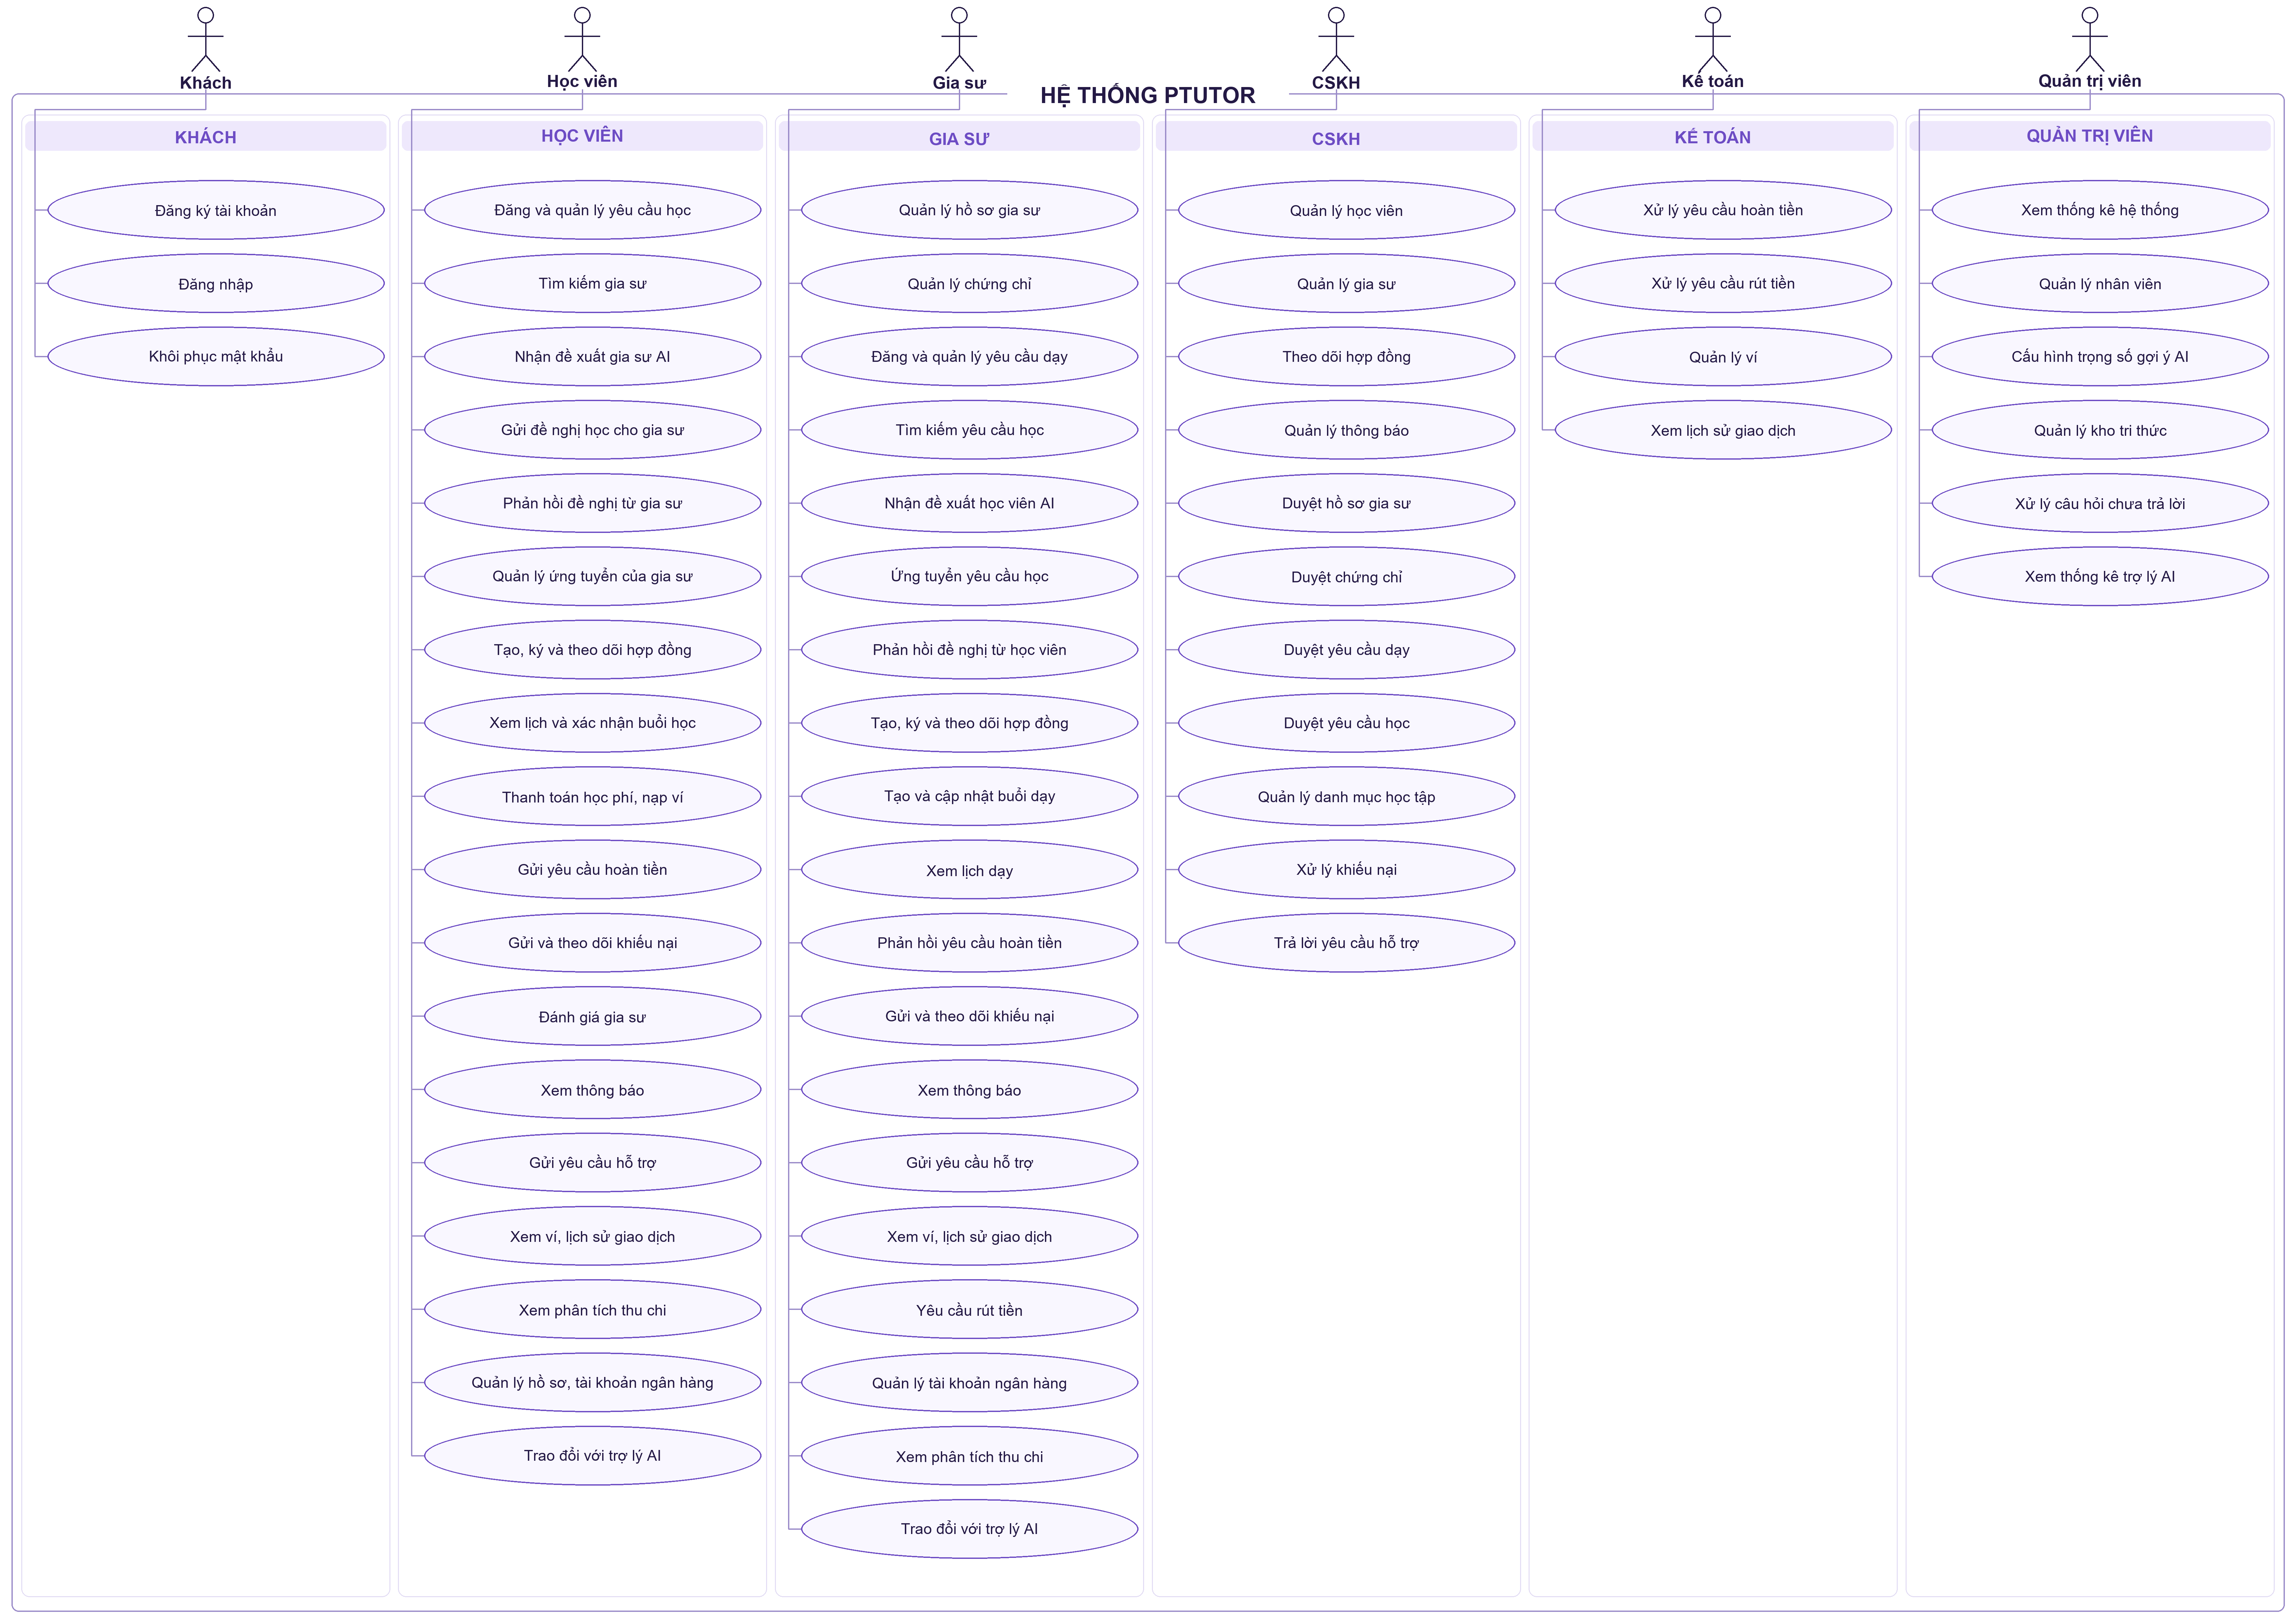
\includegraphics[width=0.96\linewidth,height=0.83\textheight,keepaspectratio]{report/diagrams/uc-tong-quan.png}
  \caption{Sơ đồ use case tổng quan hệ thống PTutor. Quản trị viên có quyền truy cập các chức năng của nhân viên chăm sóc khách hàng và kế toán.}
  \label{fig:uc-tong-quan}
\end{figure}
\end{landscape}

\begin{landscape}
\begin{figure}[p]
  \centering
  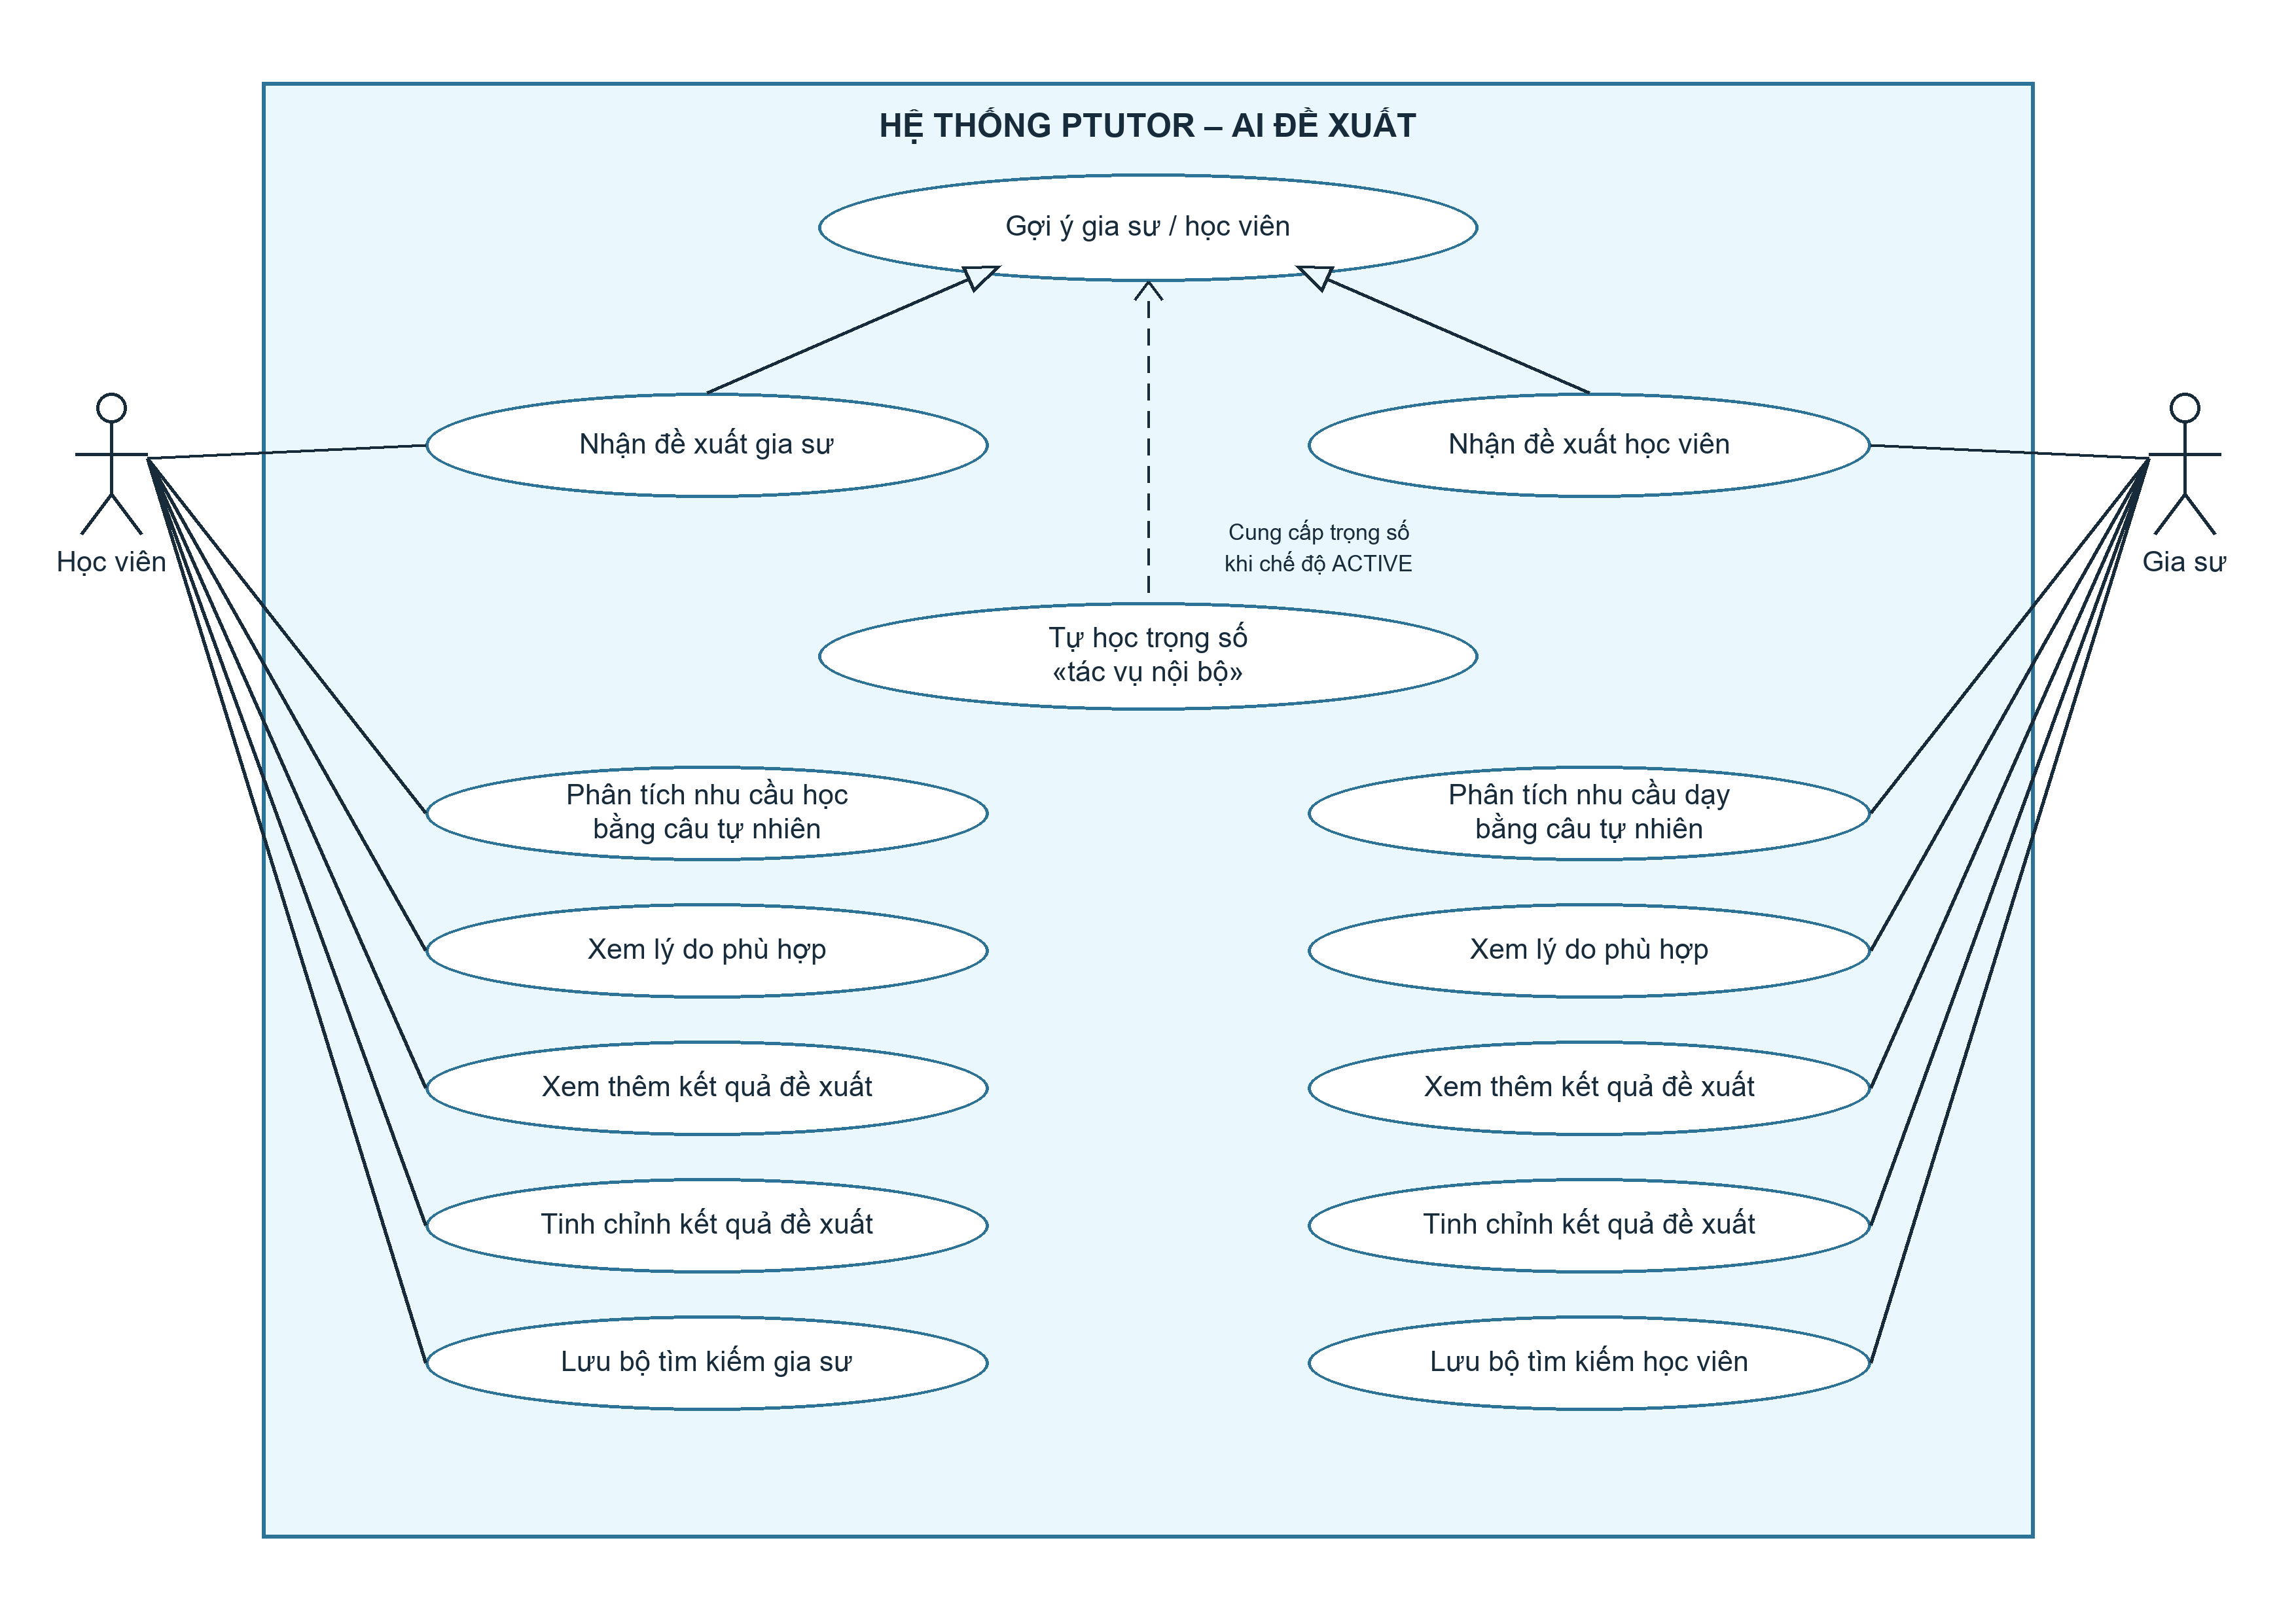
\includegraphics[width=0.96\linewidth,height=0.83\textheight,keepaspectratio]{report/diagrams/uc-ai-de-xuat.png}
  \caption{Sơ đồ use case chức năng AI đề xuất và cơ chế tự học trọng số}
  \label{fig:uc-ai-de-xuat}
\end{figure}
\end{landscape}

\begin{landscape}
\begin{figure}[p]
  \centering
  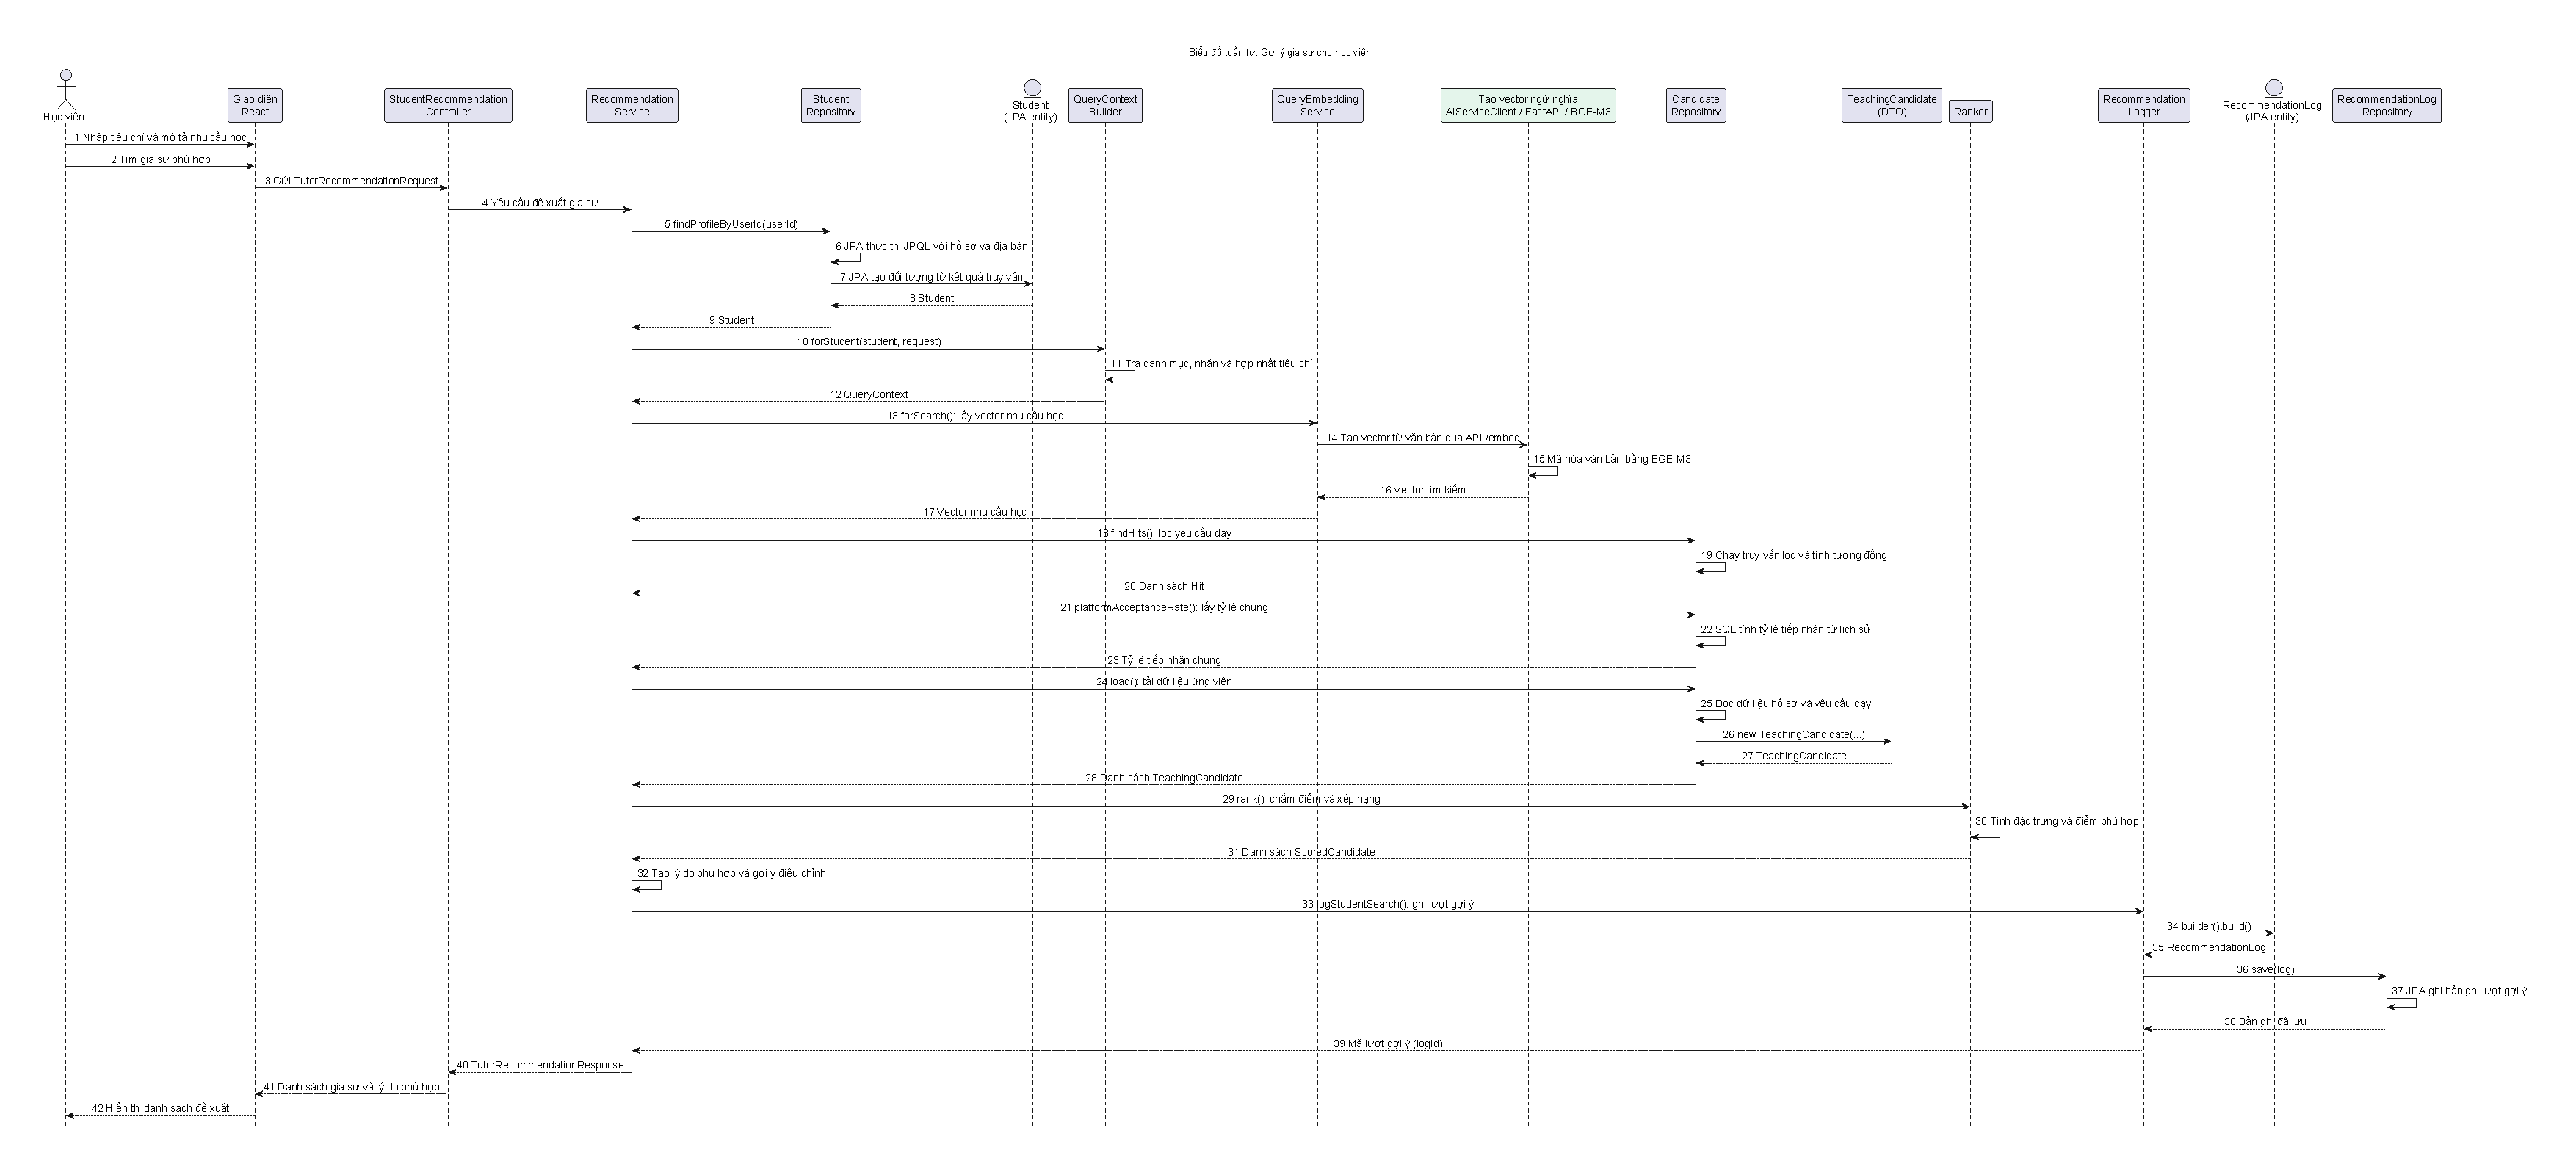
\includegraphics[width=0.96\linewidth,height=0.83\textheight,keepaspectratio]{report/diagrams/tuan-tu-goi-y-gia-su-bao-cao.pdf}
  \caption{Biểu đồ tuần tự chức năng đề xuất gia sư cho học viên}
  \label{fig:tuan-tu-ai-de-xuat}
\end{figure}
\end{landscape}

\begin{landscape}
\begin{figure}[p]
  \centering
  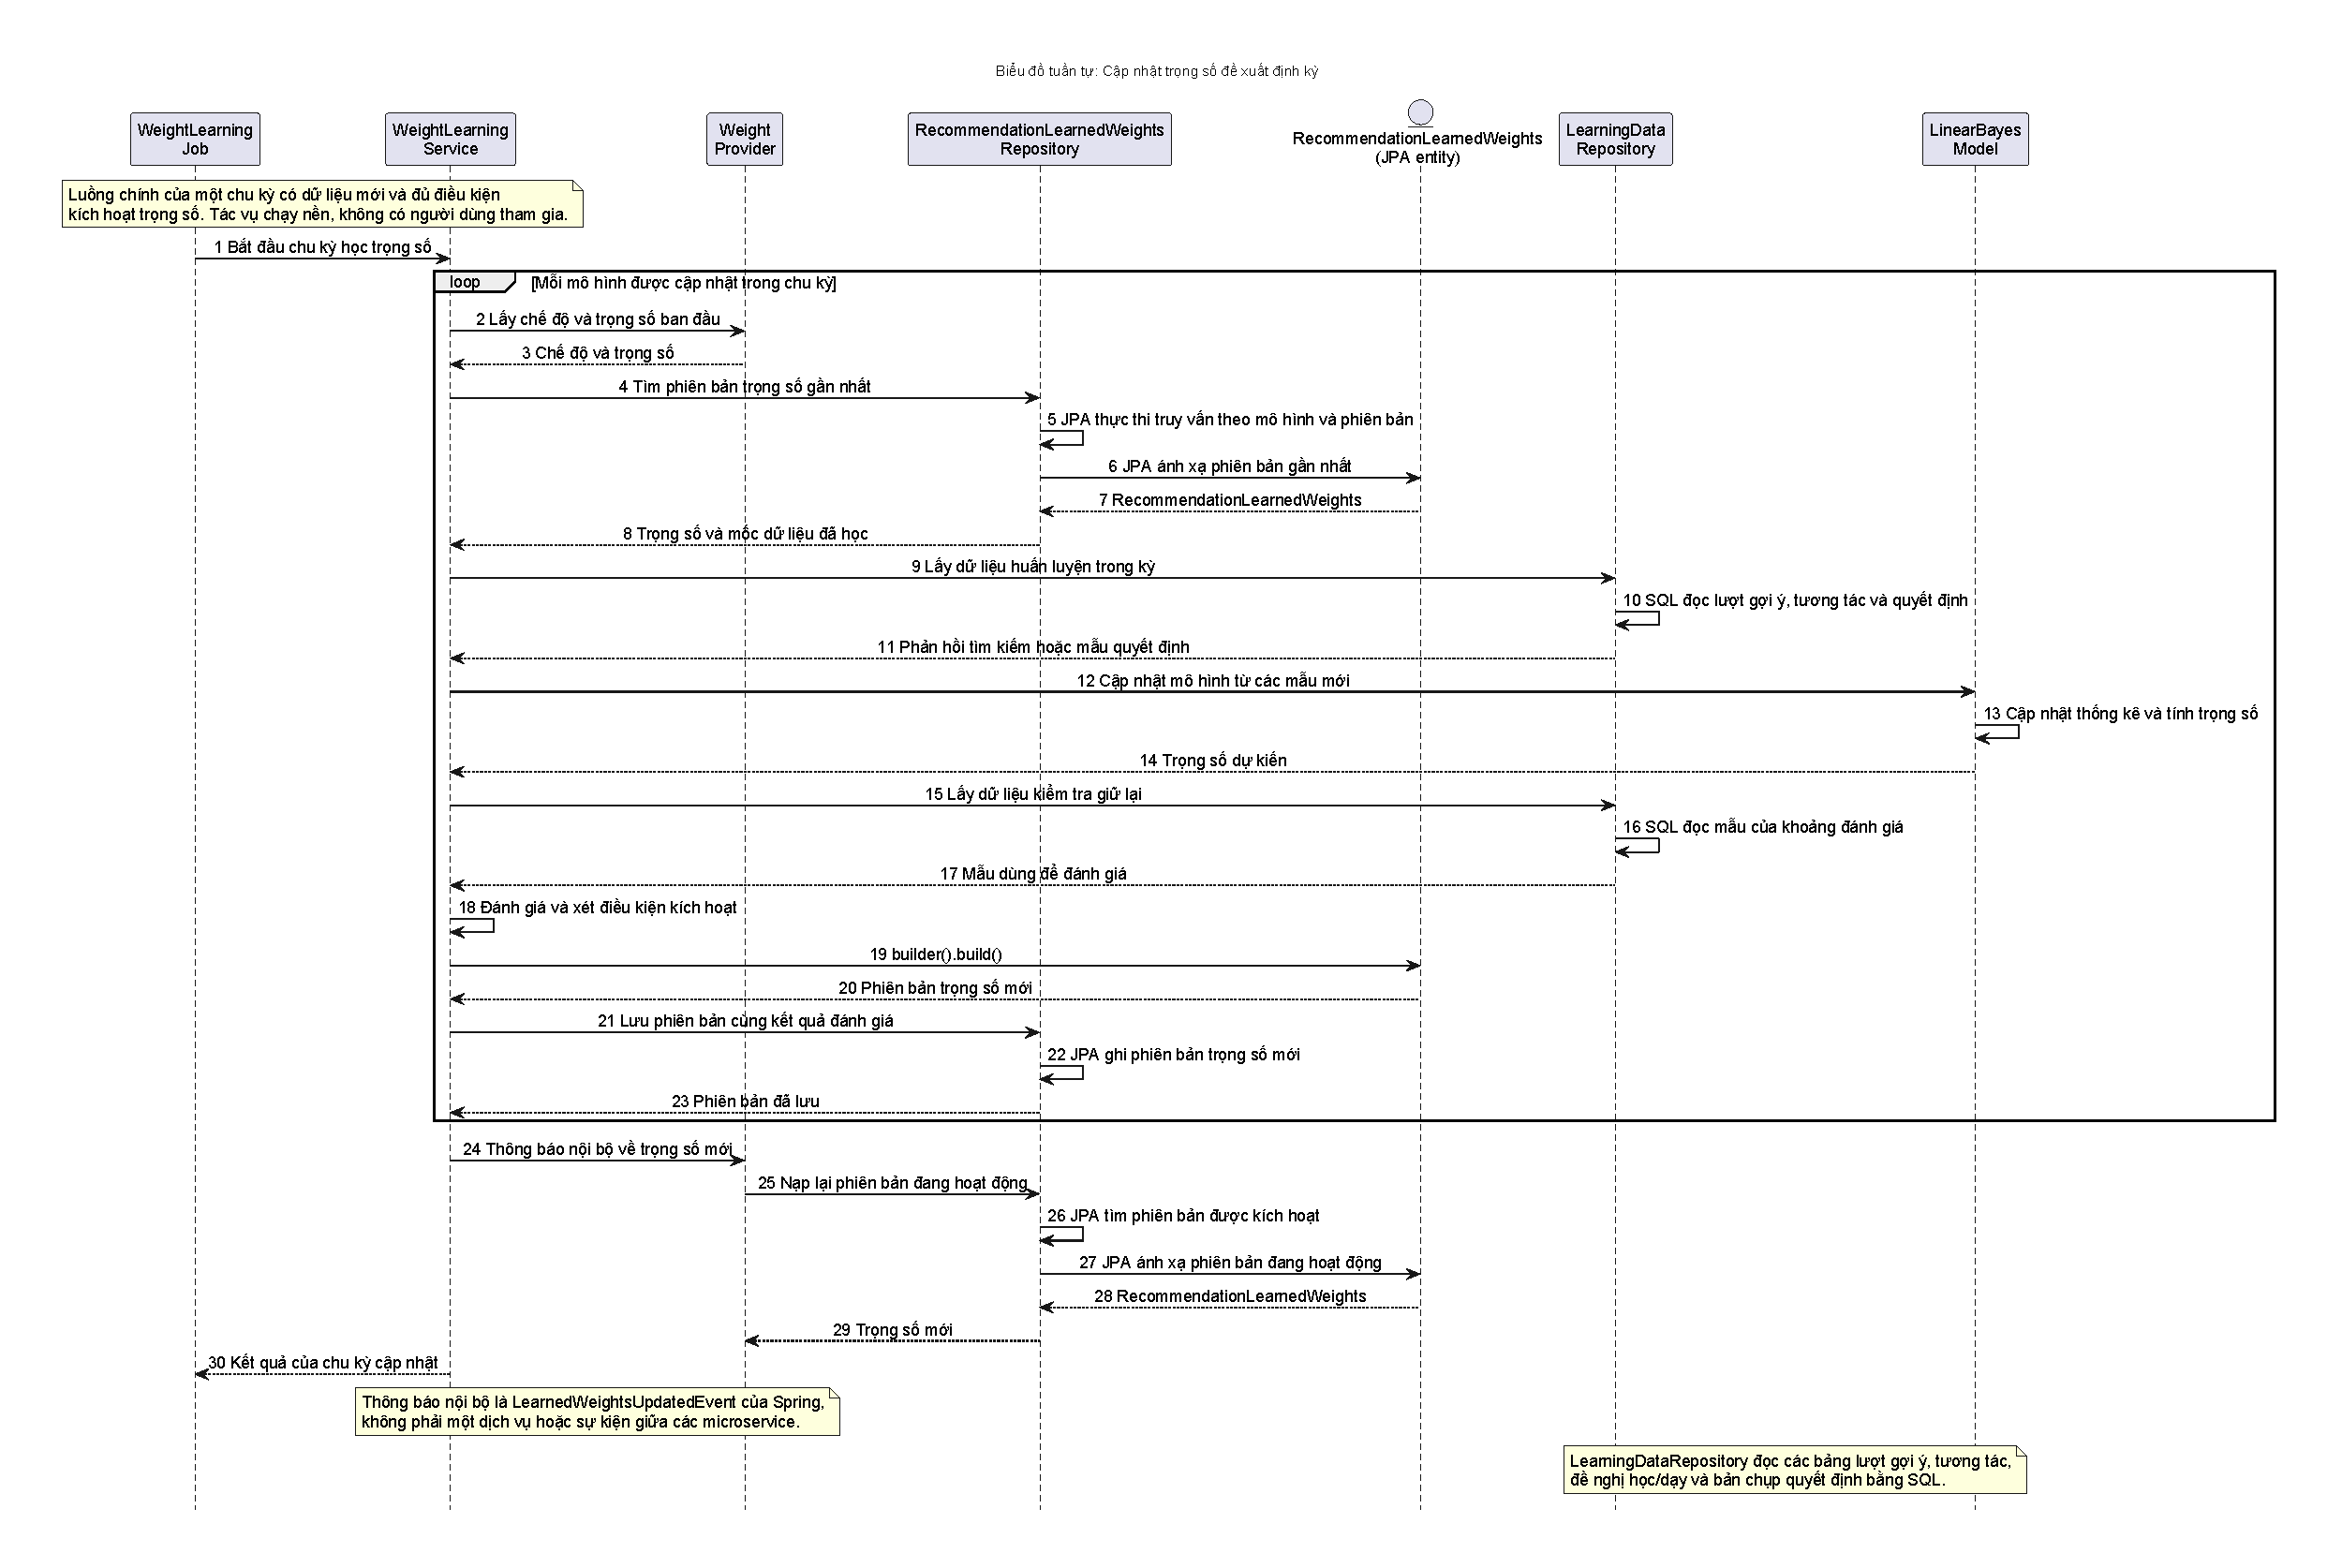
\includegraphics[width=0.96\linewidth,height=0.83\textheight,keepaspectratio]{report/diagrams/tuan-tu-tu-hoc-trong-so.pdf}
  \caption{Biểu đồ tuần tự cơ chế tự học trọng số của chức năng AI đề xuất}
  \label{fig:tuan-tu-tu-hoc-trong-so}
\end{figure}
\end{landscape}

% Đặt nội dung kich-ban-ai-de-xuat.tex tại mục mô tả kịch bản.
% Có thể dùng % Cần các gói: longtable, array, enumitem, graphicx.
% Có thể đổi số bảng theo vị trí thực tế trong báo cáo.
\begin{longtable}{|p{0.20\textwidth}|p{0.72\textwidth}|}
\caption{Kịch bản chức năng AI đề xuất đối tượng phù hợp}\label{tab:ai-de-xuat}\\
\hline
\textbf{Nội dung} & \textbf{Mô tả} \\ \hline
\endfirsthead
\hline
\textbf{Nội dung} & \textbf{Mô tả} \\ \hline
\endhead
Tên ca sử dụng & AI đề xuất gia sư cho học viên hoặc đề xuất yêu cầu học cho gia sư. \\ \hline
Tác nhân & Học viên, gia sư. \\ \hline
Mục đích & Tìm và xếp hạng các đối tượng phù hợp với môn học, khối lớp, khu vực, lịch học, học phí và nhu cầu của người tìm kiếm. \\ \hline
Tiền điều kiện & Người dùng đã đăng nhập bằng tài khoản học viên hoặc gia sư. Hồ sơ và các yêu cầu học/dạy dùng để tìm kiếm đã được hệ thống lưu trữ. \\ \hline
Hậu điều kiện & Danh sách đề xuất và lý do phù hợp được hiển thị. Hệ thống lưu lần tìm kiếm cùng thứ tự xếp hạng để phục vụ phân trang và ghi nhận tương tác. Việc xem đề xuất không tự tạo hợp đồng hay lời mời. \\ \hline
Kịch bản chính &
\begin{enumerate}[leftmargin=*,nosep]
  \item Người dùng mở trang đề xuất. Hệ thống hiển thị các bộ lọc và, nếu có, thông tin từ yêu cầu học hoặc yêu cầu dạy của người dùng.
  \item Người dùng chọn một yêu cầu đã có hoặc nhập tiêu chí tìm kiếm, sau đó kiểm tra và điều chỉnh môn học, khối lớp, khu vực, mức phí và lịch học theo nhu cầu.
  \item Người dùng gửi yêu cầu tìm kiếm. Giao diện chuyển các tiêu chí tới API đề xuất của hệ thống.
  \item Hệ thống xác thực người dùng, tổng hợp tiêu chí từ bộ lọc, yêu cầu đã chọn và hồ sơ. Nếu đã đủ thông tin bắt buộc, hệ thống tạo biểu diễn ngữ nghĩa cho nhu cầu tìm kiếm.
  \item Hệ thống truy vấn các yêu cầu dạy hoặc yêu cầu học còn hiệu lực, loại các bản ghi không đáp ứng điều kiện bắt buộc, tính điểm phù hợp và sắp xếp kết quả.
  \item Hệ thống tạo lý do đề xuất, lưu thứ tự kết quả của lần tìm kiếm và trả về danh sách đề xuất cùng mã lần tìm kiếm.
  \item Giao diện hiển thị các kết quả, thông tin liên quan và lý do phù hợp. Người dùng có thể xem chi tiết, xem thêm kết quả hoặc thực hiện bước liên hệ/ứng tuyển theo quyền của mình.
\end{enumerate} \\ \hline
Luồng thay thế &
\begin{enumerate}[leftmargin=*,nosep]
  \item[2a.] Người dùng nhập nhu cầu bằng câu tự nhiên. Hệ thống dùng mô hình ngôn ngữ để nhận diện tiêu chí, điền vào bộ lọc; người dùng xác nhận hoặc sửa trước khi thực hiện bước 3.
  \item[7a.] Người dùng chọn xem thêm. Giao diện gửi mã lần tìm kiếm và số trang; hệ thống đọc thứ tự đã lưu và trả về trang tiếp theo.
  \item[7b.] Người dùng chọn tinh chỉnh. Hệ thống cập nhật kết quả dựa trên lần tìm kiếm và các mục đã xem, sau đó trả về danh sách mới.
\end{enumerate} \\ \hline
Ngoại lệ &
\begin{enumerate}[leftmargin=*,nosep]
  \item[4a.] Thiếu môn học hoặc khối lớp cần thiết: hệ thống trả về danh sách trường cần bổ sung; người dùng cập nhật tiêu chí rồi tìm lại.
  \item[4b.] Dịch vụ tạo biểu diễn ngữ nghĩa không khả dụng: hệ thống dùng dữ liệu hồ sơ hoặc tiêu chí có sẵn để tiếp tục tìm kiếm theo cơ chế dự phòng.
  \item[5a.] Không có kết quả thỏa điều kiện: hệ thống hiển thị trạng thái rỗng và gợi ý nới lỏng các tiêu chí có thể điều chỉnh.
  \item[2b.] Không phân tích được câu tự nhiên: người dùng nhập trực tiếp trên bộ lọc và tiếp tục tìm kiếm.
\end{enumerate} \\ \hline
\end{longtable}
.
